\chapter{Contexte général du projet}
\label{chap:Contexte général du projet}



Dans ce chapitre, nous situons notre stage de fin d’études dans son environnement organisationnel et contextuel. Nous présentons d'abord l’organisme d’accueil, SQLI Maroc. Ensuite, nous détaillons la problématique qui a conduit à la réalisation de ce projet et les objectifs visés. Finalement, nous abordons la méthodologie adoptée pour la réalisation du projet.
\newpage


\section{Présentation de l’entreprise d’accueil SQLI}

Cette section initiale met en lumière le Groupe SQLI en mettant l’accent sur ses activités clés, son
chiffre d’affaires ainsi que ses clients. Ensuite, nous nous concentrerons spécifiquement sur SQLI Maroc et
ses valeurs clés.

\subsection{Groupe SQLI}

\begin{figure}[h]
    \centering
    
\includegraphics[scale=0.7]{Logos/SQLI_LOGO.png} % Replace with the actual filename of the IBM logo image
    \caption{Logo de SQLI \cite{SQLI}}
    \label{fig:LogoSQLI}
\end{figure}

SQLI est une entreprise européenne de services numériques fondée en 1990 par Jean Rouveyrol et Alain Lefebvre. Elle se spécialise dans la conception, le développement et le déploiement de solutions digitales
visant à créer des expériences unifiées \cite{SQLI}. Avec un effectif de 2400 collaborateurs répartis dans 13 pays,
SQLI bénéficie d’une présence internationale solide.

Le succès de SQLI Digital Experience repose sur des valeurs fondamentales telles que la créativité, l'engagement et l'audace visionnaire. Ces valeurs imprègnent chaque aspect de l'entreprise, permettant de repousser les frontières de l'innovation et de concevoir des expériences digitales uniques et captivantes. \cite{valeurSQLI}

\subsubsection{Activités du groupe}

Le groupe SQLI propose une gamme étendue de services pour accompagner les entreprises dans leur transformation numérique. Il inclut l'e-commerce, créant et optimisant des plateformes de vente en ligne performantes. Il offre également des plateformes d'expérience, conçues pour offrir des interactions utilisateur exceptionnelles. En matière de technologie et de transformation, il aide les entreprises à moderniser leurs infrastructures et leurs processus. Ses services de data et insights permettent d'exploiter les données de manière stratégique, tandis que son expertise en marketing digital et design améliore la visibilité et l'attrait des marques. Enfin, son conseil digital guide les entreprises dans l'élaboration et la mise en œuvre de leur stratégie numérique globale, assurant ainsi une transformation digitale réussie. \cite{SQLI}

\subsubsection{Chiffre Clés du groupe}

Les chiffres clés suivants présentent la situation actuelle de SQLI :

\begin{itemize}
    \item[$\bullet$] Fort de 33 ans d’expérience et d’innovation, SQLI fonde son développement sur une expertise technologique de pointe et une politique de veille intensive.
    \item[$\bullet$] SQLI emploie plus de 2400 collaborateurs répartis dans 13 pays, notamment la France, l'Angleterre, la Suède, les Pays-Bas, l'Espagne, l'Allemagne, la Belgique, le Luxembourg, la Suisse et le Maroc.
    \item[$\bullet$] En 2022, le groupe SQLI a atteint un chiffre d’affaires de 251,2 millions de dollars. Ce succès est le résultat d'une offre bien alignée sur les attentes du marché et d'une reprise progressive de la demande de services informatiques.
    \vspace{0.5cm}
\end{itemize}

\begin{figure}[H]
    \centering
    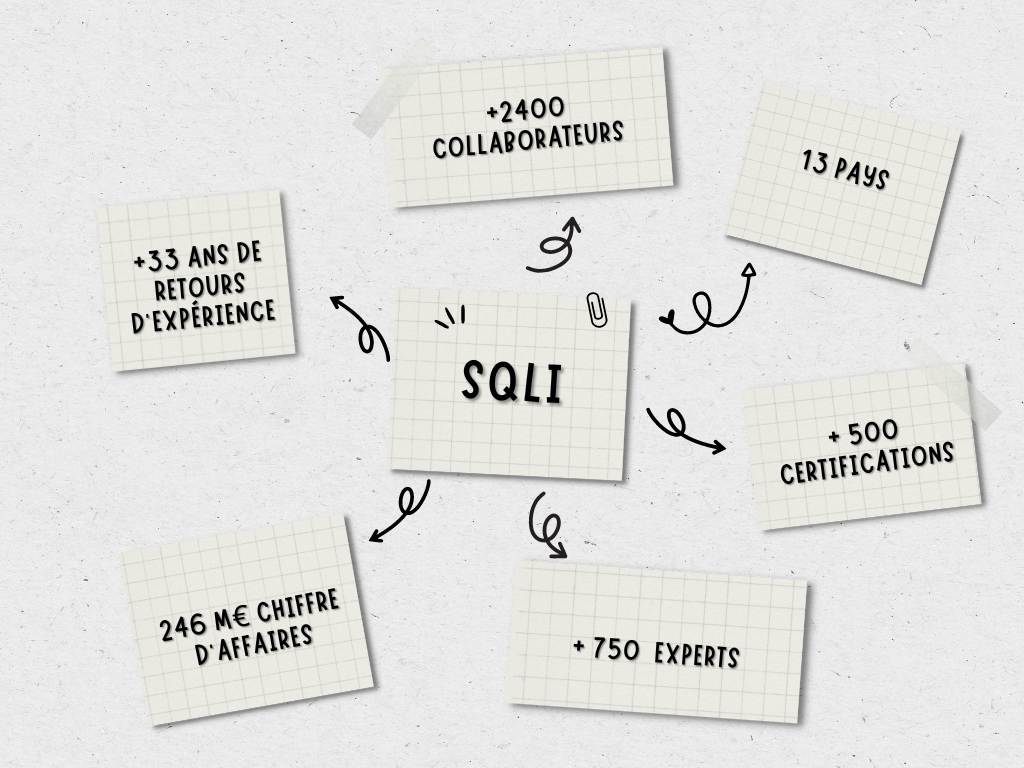
\includegraphics[width=10cm]{Figures/cle chiffre.png} % Replace with the actual filename of the IBM logo image
    \caption{Chiffre Clés de SQLI}
\end{figure}

\subsubsection{Clients du groupe}

SQLI collabore avec une vaste gamme de clients provenant de divers secteurs, y compris l'automobile, la distribution, la banque et l'assurance, le luxe et la mode, la santé, l'industrie et l'énergie, ainsi que les télécommunications. Les grandes entreprises internationales et les organisations locales font appel à SQLI pour ses solutions digitales innovantes, allant de l'optimisation des plateformes d'e-commerce à la transformation numérique des services financiers, en passant par la création d'expériences utilisateur uniques pour les marques de luxe et la digitalisation des processus industriels. Grâce à sa capacité à répondre aux besoins spécifiques de chaque secteur, SQLI bâtit des partenariats solides et durables avec ses clients

\begin{figure}[H]
    \centering
    
\includegraphics[width=15cm]{Figures/sqli partenaire .png} % Replace with the actual filename of the IBM logo image
    \caption{Clients du SQLI \cite{SQLI}}
\end{figure}


\subsection{SQLI Maroc}

SQLI Maroc, créée en 2003 à Rabat par Eric Chanal, représente le centre de Delivery et d'Innovation du Groupe SQLI. Bénéficiant d'une solide expertise et d'une grande expérience, l'entreprise est présente sur trois sites stratégiques : Rabat, où nous avons eu l'opportunité d'effectuer notre stage PFE, Oujda et Casablanca.   Voici sa fiche technique:



% l'ajoute de titre de tableau avec space between titre de tab et le tab
% \captionsetup{type=table}

% \vspace{0.3cm}
% tab
\begin{center}
    \captionsetup{type=table}
    \captionof{table}{Fiche technique de SQLI Maroc}
    \vspace{0.3cm}
    \begin{tabularx}{17cm}{|X|X|}
      \hline
     \textbf{Dénomination sociale}  & \textbf{SQLI Digital Experience} \\
      \hline
     {Année de fondation} & 2003  \\
      \hline
      {Fondateur} & Eric Chanal  \\
      \hline
     {Siège social} & Rabat, Maroc\\
     \hline  
     {Activité} & Conseil en systèmes et logiciels informatiques.\\
      \hline  
     {Effectif des employés} & Plus de 900 collaborateurs.\\
      \hline
     {Sites d'implantation} & Rabat, Oujda et Casablanca.\\
      \hline
     {Site web} & https://www.sqli.com/fr-fr\\
      \hline
     {Téléphone} & Pour le bureau de Rabat : +212 537 619 710 \\
      \hline
    \end{tabularx}
    \end{center}
    

  SQLI Maroc comprend principalement deux structures essentielles, à savoir :

\begin{enumerate}
    \item \textbf{SQLI WAX INTERRACTIVE} : S’occupe à accompagner les clients sur la voie de digitalisation afin d’avoir un bon positionnement sur le marché. Cette structure
     intervient sur le plan stratégique vis-à-vis les clients.
     \item \textbf{SQLI ENTREPRISE} : Cette entité est chargée de la mise en œuvre des systèmes d'information pour les clients. Elle se compose de plusieurs Business Units spécialisées dans différents domaines :
\begin{itemize}

    \item \textbf{E-commerce/ JAVA EE} : se focalise sur la création et la mise en place de sites de e-commerce ainsi que sur le développement d'applications utilisant la technologie JAVA EE.
    \item \textbf{Mobile/Front} : spécialise dans le développement d'applications mobiles et de l'interface utilisateur (Front-end) pour les clients.
     \item \textbf{Microsoft} : se charge de la réalisation d'applications basées sur les technologies Microsoft.
      \item \textbf{Agency} : joue un rôle transversal en assurant la conception de l'interface utilisateur (Front-end) pour toutes les autres Business Units.
        \item \textbf{Delivery} : se charge de la gestion des livraisons et des recettes vis-à-vis des clients.       
\end{itemize}
\end{enumerate}
\vspace{0.5cm}
\begin{figure}[H]  
  \centering  
  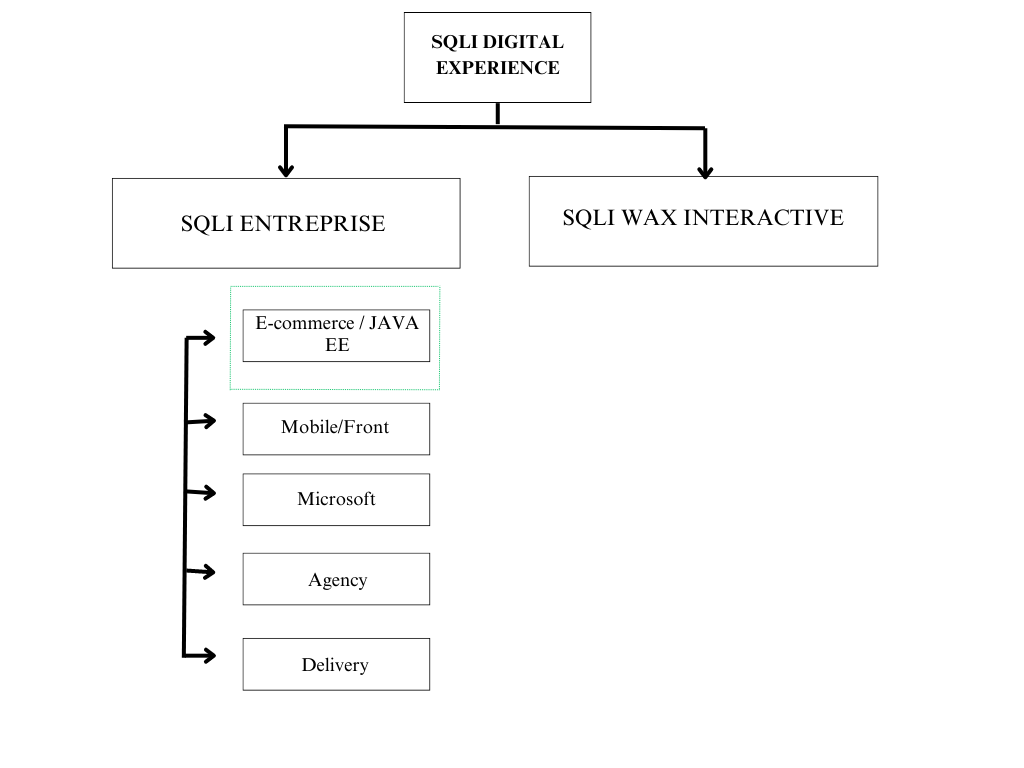
\includegraphics[width=14cm]{Figures/departement.png}
  \caption{Départements de SQLI}
  \label{Over The Air updates}
\end{figure}


Notre stage de fin d'études s'est déroulé dans le département Java JEE, qui regroupe plusieurs projets destinés à de grandes entreprises clientes.


\section{Présentation du projet}

\subsection{Cadre du projet et problématique}

Dans le cadre d'un projet e-commerce pour un client, l'objectif est d'améliorer et d'optimiser sa plateforme actuelle. Il est indispensable de mettre à jour régulièrement cette plateforme, qui joue un rôle crucial dans les activités commerciales en ligne du client, afin de maintenir sa compétitivité et de répondre aux exigences du marché.

Pour cette amélioration, le travail inclut la correction de divers bugs qui affectent la performance et la fiabilité du système. La résolution de ces bugs est cruciale pour garantir une expérience utilisateur fluide et sans interruptions.

En parallèle, l'intégration de nouvelles fonctionnalités est nécessaire pour enrichir l'offre de la plateforme. L'un des changements majeurs est l'intégration de la méthode de paiement Payconiq, destinée spécifiquement au marché belge. Différents défis se posent lors de cette intégration, tels que la compatibilité avec l'architecture existante, la gestion des dépendances et l'assurance que cette nouvelle fonctionnalité ne provoque pas de régressions ou de nouveaux bugs.

L'enjeu majeur consiste donc à corriger les bugs existants tout en intégrant Payconiq de manière efficace, en maintenant la stabilité et la performance globale de la plateforme.

 \subsection{Objectifs du projet}

Dans le contexte de la croissance rapide de l'entreprise 4D Logiciel et de l'évolution constante du paysage technologique, la gestion efficace des formations est devenue une priorité stratégique. Pour répondre à cette demande croissante et garantir le développement continu des compétences de son personnel et de ses clients, 4D Logiciel entreprend le développement d'une plateforme interne de gestion des formations. Les objectifs de ce projet sont les suivants :

\begin{itemize}
    \item[$\bullet$] \textbf{Développer une plateforme interne de gestion des formations :} 
    
    Créer une plateforme dédiée qui permettra à 4D Logiciel de gérer efficacement tous les aspects de ses programmes de formation, depuis la planification jusqu'à la diffusion des cours.

    \item[$\bullet$] \textbf{Centraliser les formations :} 
    
    Réunir toutes les formations dispensées aux employés et aux clients au sein d'une seule plateforme pour une gestion plus cohérente et simplifiée.

    \item[$\bullet$] \textbf{Personnaliser l'expérience de formation :} 
    
    Offrir une expérience de formation personnalisée en proposant des cours adaptés aux besoins spécifiques des employés et des clients de 4D Logiciel.

    \item[$\bullet$] \textbf{Réduire les coûts associés aux formations :} 
    
    Diminuer les dépenses liées à l'achat d'abonnements sur des plateformes externes en développant une solution interne plus rentable sur le long terme.

    \item[$\bullet$] \textbf{Fournir des outils d'analyse et de suivi :} 
    
    Intégrer des fonctionnalités d'analyse et de suivi des progrès des apprenants pour évaluer l'efficacité des programmes de formation et identifier les domaines nécessitant des améliorations.
   
    \item[$\bullet$] \textbf{Assurer la sécurité des données :} 
    
    Garantir la sécurité des données des utilisateurs et des contenus de formation en mettant en place des mesures de protection appropriées.

\end{itemize}

 %%%%%%%%%%%%%%%%%%%% SECTION 4 %%%%%%%%%%%%%%%%%%%%%%%
\section{Conduite de projet}

\subsection{Equipe Cart, Checkout \&\ Payment}

Après la période de formation, j'ai intégré l'équipe Seasonal Event du projet Chanel One en tant que stagiaire backend. Cette équipe est responsable de tout ce qui concerne la recherche, les lunettes et la mode pour le projet Chanel. À mon arrivée, l'équipe travaillait sur le périmètre du Plan 99.5, qui avait pour objectif d'analyser les bugs, de nettoyer les logs, de corriger les erreurs et de refactoriser le code, entre autres tâches.

En travaillant avec cette équipe, j'ai constaté que j'avais du temps supplémentaire pour apprendre de nouvelles choses. J'ai donc discuté avec le team lead pour intégrer une autre équipe, Cart, Checkout \&\ Payment. Cette équipe se charge de l'intégration des nouvelles méthodes de paiement pour les différents marchés du client.

Ces deux équipes font partie d'un projet plus vaste, comprenant 15 équipes fonctionnelles différentes. Chacune de ces équipes est composée d'un Scrum Master, d'un expert technique, d'un Product Owner, d'un développeur frontend et de deux responsables qualité, favorisant ainsi le développement d'une solution robuste et performante.

La structure de l'équipe est illustrée dans le schéma ci-dessous :


\begin{figure}[h]
    \centering
    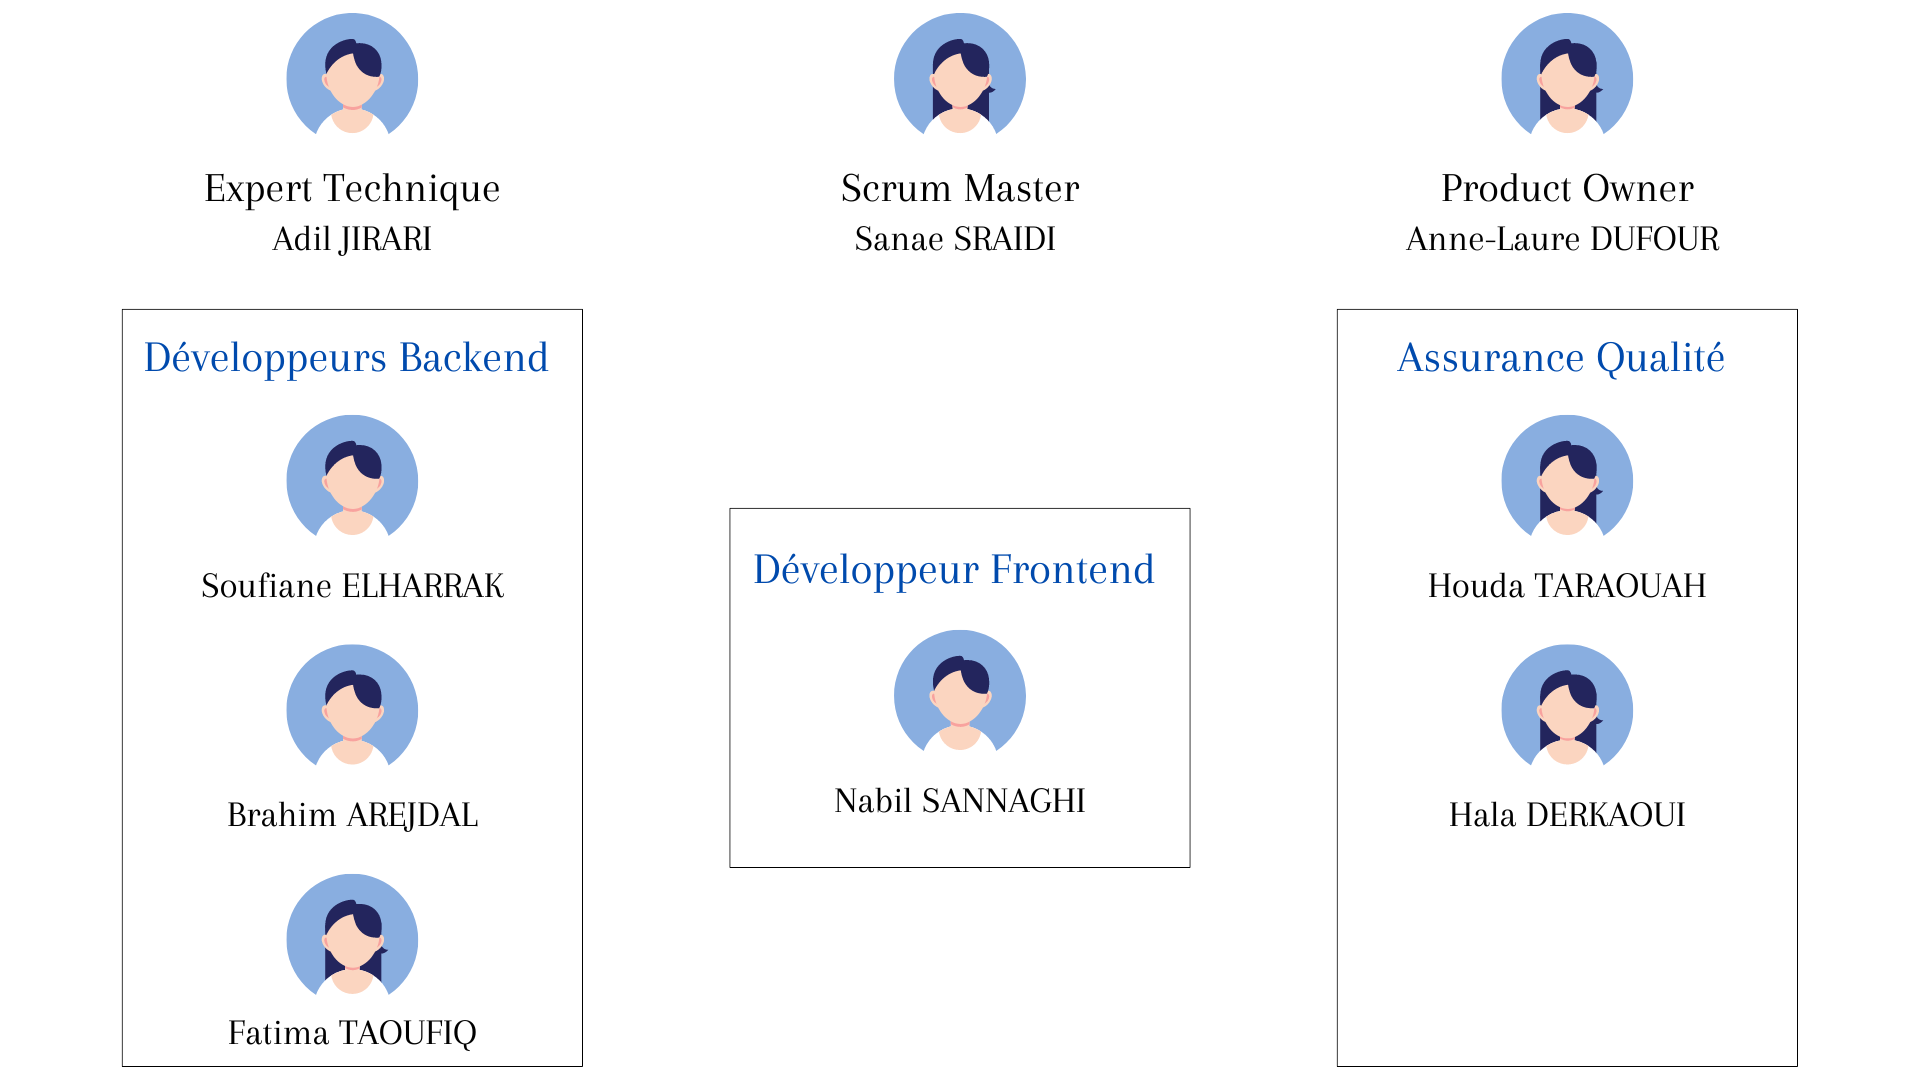
\includegraphics[width=19cm]{Figures/Cart Checkout & Payment.png} % Replace with the actual filename of the IBM logo image
    \caption{ Structure de l’équipe Cart, Checkout and Payment}
\end{figure}
\subsection{Méthodologie de travail : Scrum}

Pour assurer une collaboration efficace au sein de l'équipe, nous avons opté pour la méthodologie Scrum, qui se caractérise par une approche itérative et incrémentale. Scrum nous permet de diviser le travail en sprints, des cycles de développement courts et cadencés, généralement de deux à quatre semaines. À la fin de chaque sprint, une version potentiellement livrable du produit est présentée, ce qui favorise la flexibilité et l'adaptation aux changements. Grâce à cette méthode, nous pouvons rester réactifs et ajuster rapidement notre travail en fonction des évolutions des besoins métiers. En intégrant les retours d'expérience du client à chaque itération, nous assurons une satisfaction optimale de ses attentes. Les rôles bien définis, tels que le Scrum Master, le Product Owner, et l'équipe de développement, garantissent une communication claire et une responsabilité partagée. Cette approche nous permet d'être efficaces tout en maintenant un rythme de travail soutenu et structuré.


% \begin{itemize}
%     \item[\textbf{\textit{Planification du sprint (Sprint Planning)}}]
    
%     Avant de débuter chaque sprint, nous tenons une réunion de Sprint Planning. Cette réunion a pour objectif de définir les tâches prioritaires à accomplir au cours du sprint à venir. L'équipe, en collaboration avec le Product Owner, examine le backlog du produit pour identifier les éléments les plus critiques à traiter. Durant cette session, nous discutons des exigences, des objectifs du sprint, et nous évaluons la charge de travail nécessaire pour chaque tâche. Cette planification permet à l'équipe de se concentrer sur un ensemble de fonctionnalités claires et réalisables, tout en s'assurant que les ressources sont allouées de manière optimale. Ainsi, chacun sait précisément sur quoi se concentrer, ce qui contribue à une exécution efficace et coordonnée du sprint.
    
%     \item[\textbf{\textit{Mêlée quotidienne (Daily Meetings)}}]
    
%     Chaque jour, nous tenons une réunion appelée Daily Meeting, d'une durée de 15 minutes chaque matin. Lors de cette réunion, chaque membre de l'équipe partage ce qu'il a accompli la veille, ce qu'il prévoit de faire aujourd'hui, et signale s'il rencontre des problèmes ou des blocages. Cette réunion permet à l'équipe de rester synchronisée et d'identifier rapidement les obstacles éventuels, favorisant ainsi une meilleure collaboration et une résolution rapide des problèmes.
    
% \end{itemize}

\begin{sidewaysfigure}
    \centering
    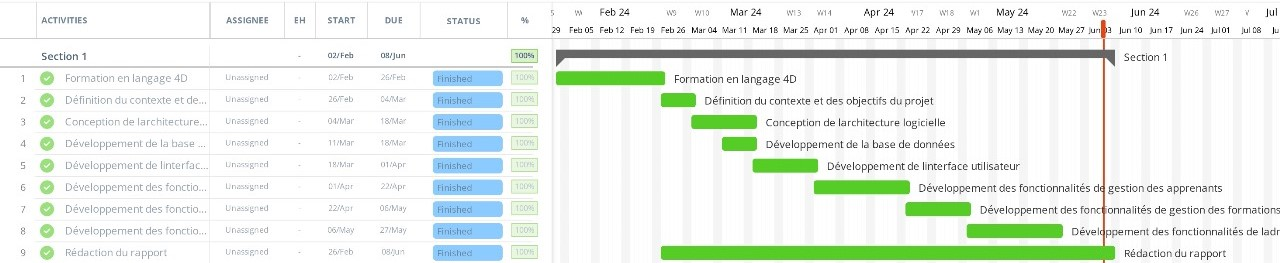
\includegraphics[width=\textheight,height=\textwidth,keepaspectratio]{Figures/DiagrammeDeGantt.jpg}
    \caption{Diagramme de Gantt.}
\end{sidewaysfigure}

\newpage
\subsection{Outils de collaboration:}

\subsubsection{Skype}

\begin{figure}[h]
    \centering
    
\includegraphics[scale=0.02]{Logos/Skype-Logo.png} % Replace with the actual filename of the IBM logo image
    \caption{Skype Logo}
\end{figure}

Skype est un logiciel propriétaire qui permet aux utilisateurs de passer des appels téléphoniques ou vidéo via Internet, ainsi que le partage d'écran. Les appels d’utilisateur à utilisateur sont gratuits, tandis que ceux vers les lignes téléphoniques fixes et les téléphones mobiles sont payants. Il existe des fonctionnalités additionnelles comme la messagerie instantanée, le transfert de fichiers et la visioconférence. 

Grâce à Skype, j'ai pu rester en contact régulier avec mon encadrant, mes collègues et les membres de l'entreprise. De plus, la fonction de partage d'écran de Skype a été extrêmement utile pour effectuer des présentations et des démonstrations de mon travail. Grâce à Skype, j'ai pu maintenir une communication fluide et efficace, ce qui a grandement contribué à la réussite de mon projet de fin d’étude.

\subsubsection{Git}

\begin{figure}[H]
    \centering
    
\includegraphics[scale=0.5]{Logos/git.png}
    \caption{Logo Git}
\end{figure}

Dans notre cas, et afin de conserver nos différentes versions du code source, nous avons
choisi de travailler avec Git comme logiciel de gestion de versions.

Git est un logiciel libre qui appartient au domaine publique (Licence GNU) et qui a
actuellement une communauté englobant près de 96\% des développeurs à travers le monde.

\subsubsection{GitLab}


\begin{figure}[H]
    \centering
    
\includegraphics[scale=0.1]{Logos/gitlab.jpg}
    \caption{Logo GitLab}
\end{figure}

Nous avons aussi opté pour GitLab, une plate-forme d'hébergement de code pour le
contrôle de version et la collaboration. Il permet, à nous et à d'autres, de travailler ensemble sur
des projets où que nous soyons.

\begin{figure}[H]
    \centering
    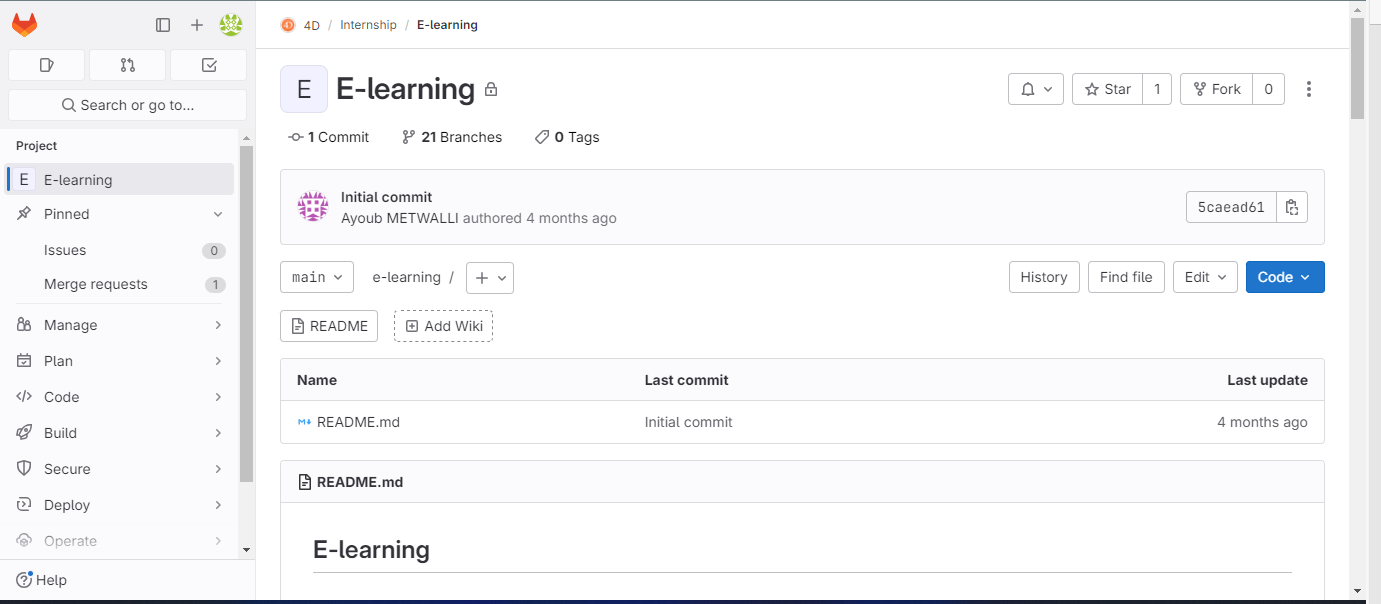
\includegraphics[width=19cm]{Figures/apercu.png}
    \caption{Aperçu globale de l'espace GitLab}
\end{figure}
\newpage

\section*{Conclusion}
Au cours de ce chapitre, nous avons mis l’accent sur le périmètre de notre projet. Nous avons éclairé
la méthodologie et le planning suivis pour mener ce projet. Nous entamerons dans le chapitre suivant
la phase d’analyse et spécification du système à développer au cours de laquelle nous comprenons en
profondeurs les besoins utilisateurs et construisons ainsi un système qui y répond.

